%
% problemstellung.tex -- Beispiel-File für die Beschreibung des Problems
%
% (c) 2020 Prof Dr Andreas Müller, Hochschule Rapperswil
%
\section{Problemstellung
\label{legendre:section:problemstellung}}
\rhead{Problemstellung}
Die zugeordneten Legendre-Polynome sind die Lösungen der allgemeinen {\em Legendre-Gleichung}
% Legendre-gleichung
\index{Legendre-Gleichung}
\begin{equation}
(1-x^2) \frac{d^2y}{dx^2}
-2x \frac{dy}{dx}
+ \left[ l(l+1)- \frac{m^2}{1-x^2} \right] y
=0
\label{legendre:legendregleichung}
\end{equation}
\cite{legendre:assoc-legendre-poly-wolfram} \cite{legendre:assoc-legendre-diff-wolfram}.
Die Lösung dieser Gleichung lässt sich mittels Polynomansatz
% Polynomansatz
\begin{equation}
y(x)=a_0+a_1x+ \ldots + a_nx^n
\label{legendre:polynomansatz}
\end{equation}
\index{Polynomansatz}%
finden und führt auf die geschlossene Form \eqref{legendre:geschlosseneform} aus Abschnitt \ref{legendre:section:einleitung}.
Die zugeordneten Legendre-Polynome sind zudem nur auf dem Intervall $[-1, 1]$ definiert.
Verwendung finden diese Polynome vor allem als Teil der Kugelflächenfunktionen (engl. {\em spherical harmonics}) \cite{legendre:spherical-harmonic-wolfram}.
\index{spherical harmonics}%

Ein zugeordnetes Legendre-Polynom wird mit $P^m_l$ bezeichnet und besitzt zwei Parameter, $l$ und $m$.
Dabei gilt für die beiden Parameter, dass $l\geq 0$ und $m=0, \ldots , l$.
Der Parameter $l$ ist für den Grad des zugeordneten Legendre-Polynoms verantwortlich, $m$ hingegen wird mancherorts, für Polynome eher ungewöhnlich, als {\em Ordnung} des Polynoms bezeichnet.
Aus den Bedingungen für die beiden Parameter $l$ und $m$ ergibt sich eine Struktur möglicher zugeordneter Legendre-Polynome.
Der Anfang dieser Struktur ist in Abbildung \ref{legendre:fig:struktur} dargestellt.
% Plot Legendre-polynome Struktur
\begin{figure}[!ht]
\centering
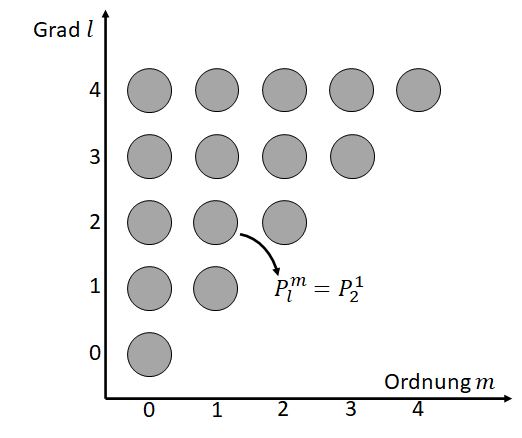
\includegraphics[width=0.6\linewidth]{papers/legendre/plots/legendre_struktur}
\caption{Ausschnitt aus der Struktur der möglichen zugeordneten Legendre-Polynome.}
\label{legendre:fig:struktur}
\end{figure}

Wie im Abschnitt \ref{legendre:section:einleitung} bereits erwähnt, gibt es Rekursionsbeziehungen für die zugeordneten Legendre-Polynome.
\index{Rekursionsbeziehung}%
Der englische Wikipedia-Artikel \cite{legendre:wikipedia} zu den zugeordneten Legendre-Polynomen führt eine Liste solcher Rekursionsformeln.
Die ersten beiden Rekursionsformeln des Wikipedia-Artikels sind wohl die gängigsten.
Die erste Rekursionsformel
% Rekursionsformel in l-Richtung
\begin{equation}
(l-m+1)P^{m}_{l+1}(x)
=(2l+1)xP^{m}_{l}(x)
-(l+m)P^{m}_{l-1}(x)
\label{legendre:recurrence-l}
\end{equation}
verläuft in der Richtung des Parameters $l$, also in der Richtung des Grades des Legendre-Polynoms.
Diese Rekursionsbeziehung nennen wir ab jetzt $l$-Rekursion.
\index{$l$-Rekurions@l-Rekursion}%
Die zweite Rekursionsformel
% Rekursionsformel in m-Richtung
\begin{equation}
2mxP^{m}_{l}(x)
=-\sqrt{1-x^2}
\left[ P^{m+1}_{l}(x) + (l+m)(l-m+1)P^{m-1}_{l}(x) \right]
\label{legendre:recurrence-m}
\end{equation}
hingegen verläuft in der Richtung des Parameters $m$.
Analog zur vorherigen Rekursionsbeziehung nennen wir diese $m$-Rekursion.
\index{$m$-Rekursion@m-Rekursion}%
Zu erwähnen ist noch, dass die $m$-Rekursion in negativer $m$-Richtung verläuft, also in Richtung abnehmender $m$-Werte.
Dies führt dazu, dass die $m$-Rekursion nicht wie in Gleichung \eqref{legendre:recurrence-m} dargestellt verwendet werden kann.
Sie muss daher nach $P^{m-1}_{l}(x)$ aufgelöst werden.
Darauf wird später noch etwas genauer eingegangen.

Beim Erstellen der Graphen (siehe Abbildung \ref{legendre:fig:plot-l} und Abbildung \ref{legendre:fig:plot-m}) mittels diesen beiden Rekursionsformeln fällt auf, dass keine numerischen Instabilitäten ersichtlich sind, wie dies beim Graphen von Wolfram Alpha der Fall ist (vergleiche Abbildung \ref{legendre:fig:wolframalpha}).
% Plot in l-Richtung
\begin{figure}[!ht]
\centering
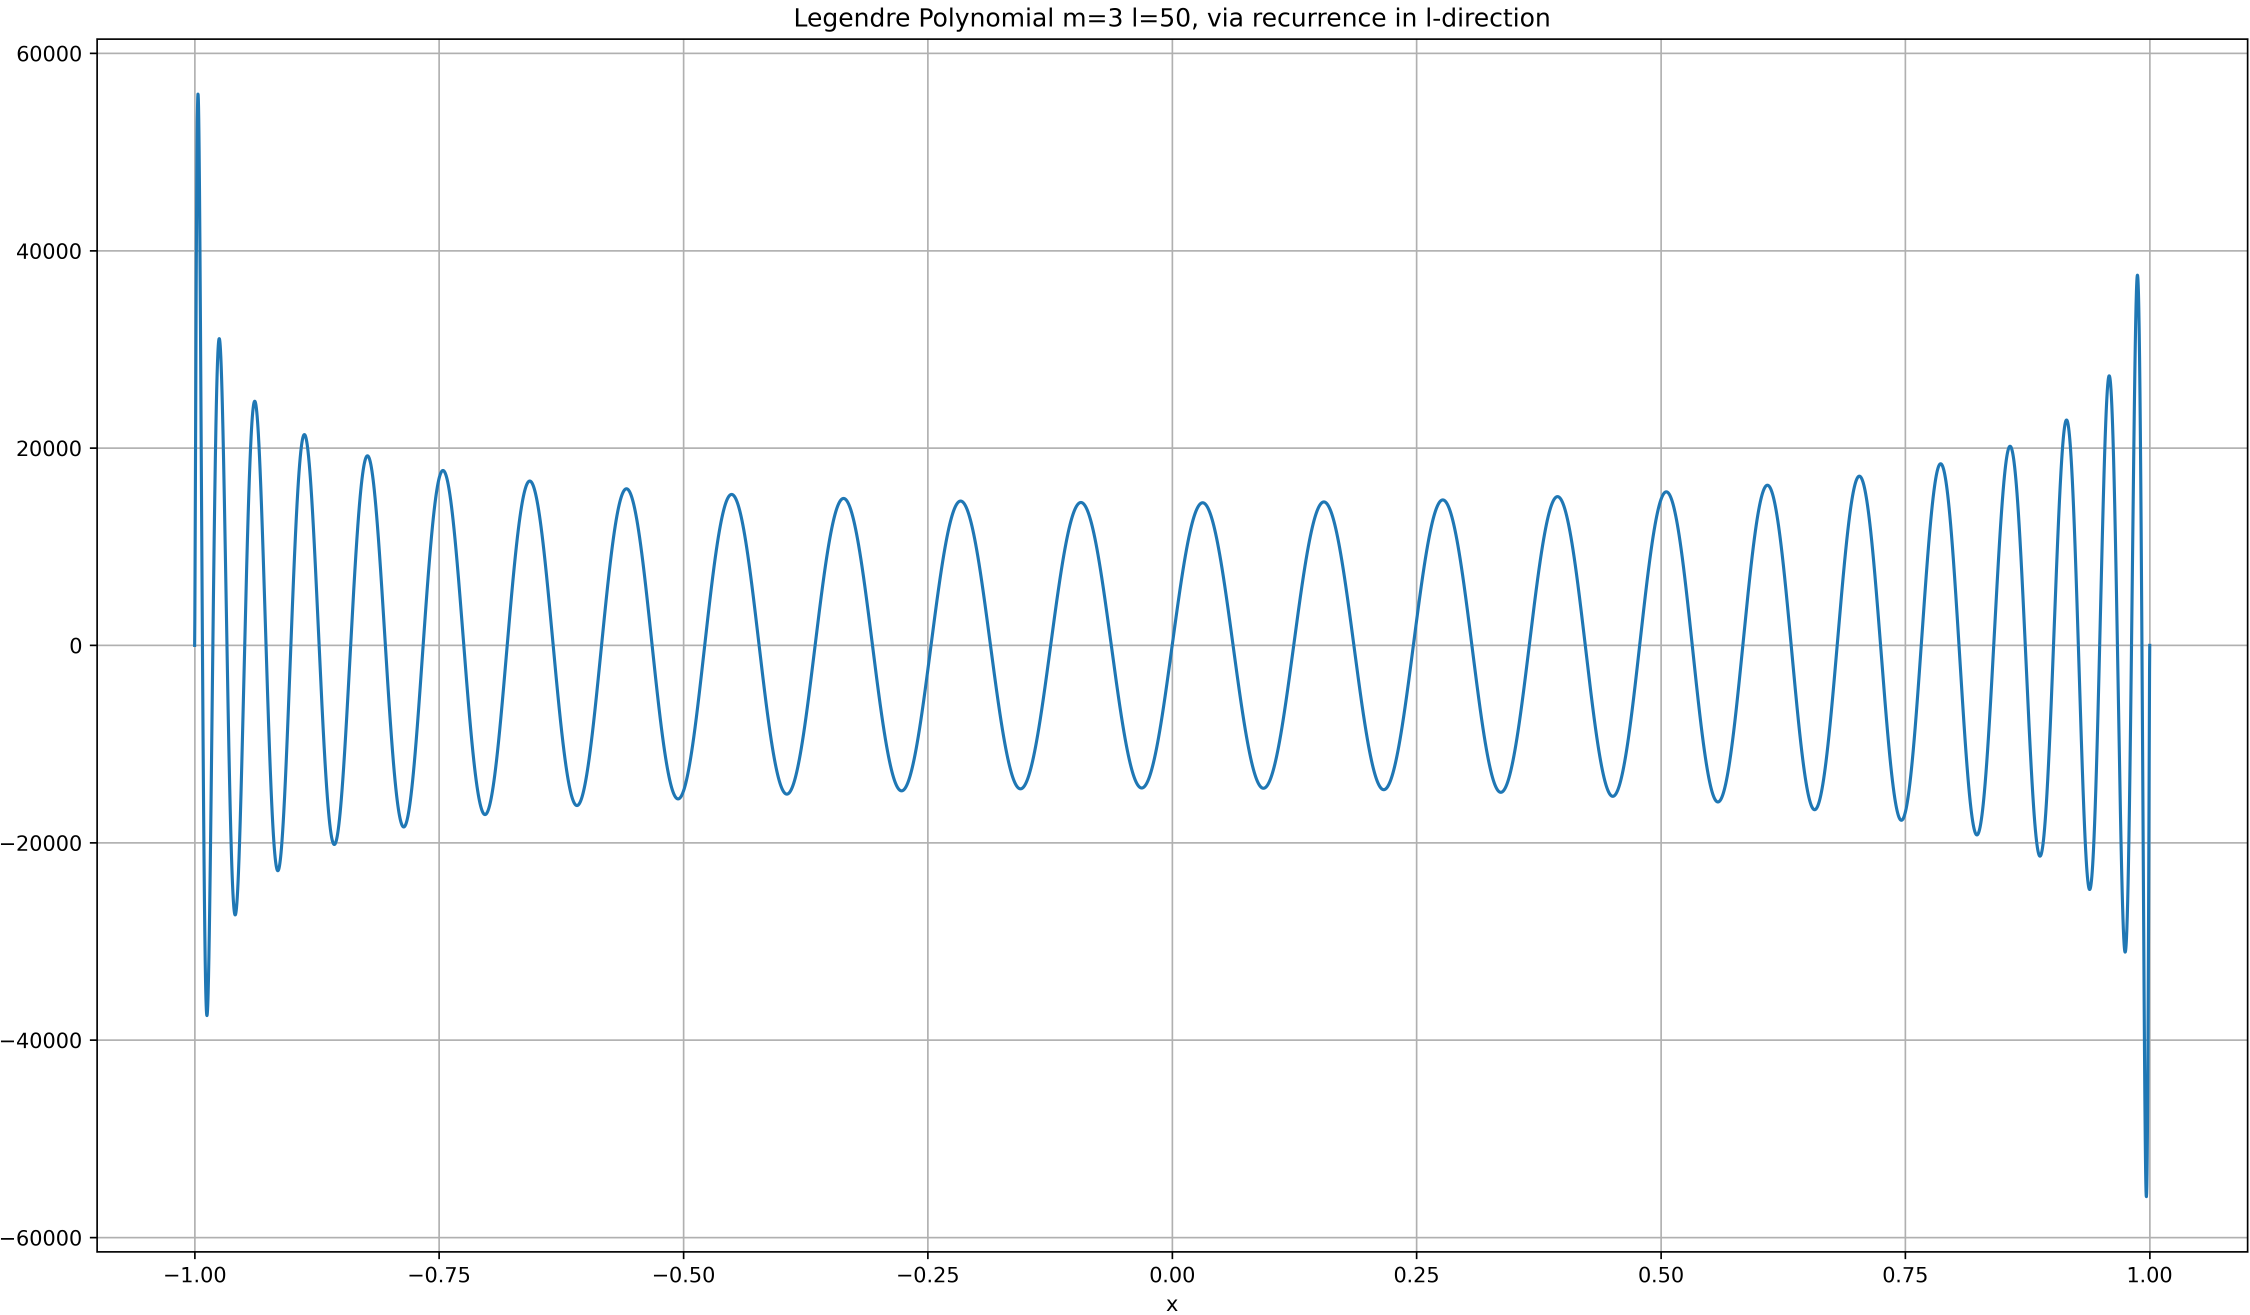
\includegraphics[width=1.0\linewidth]{papers/legendre/plots/plot_l_small.png}
\caption{Zugeordnetes Legendre-Polynom mit \texorpdfstring{$l=50$}{l=50} und \texorpdfstring{$m=3$}{m=3}, berechnet mit der Rekursionsformel in \texorpdfstring{$l$}{l}-Richtung.}
\label{legendre:fig:plot-l}
\end{figure}
% Plot in m-Richtung
\begin{figure}[!ht]
\centering
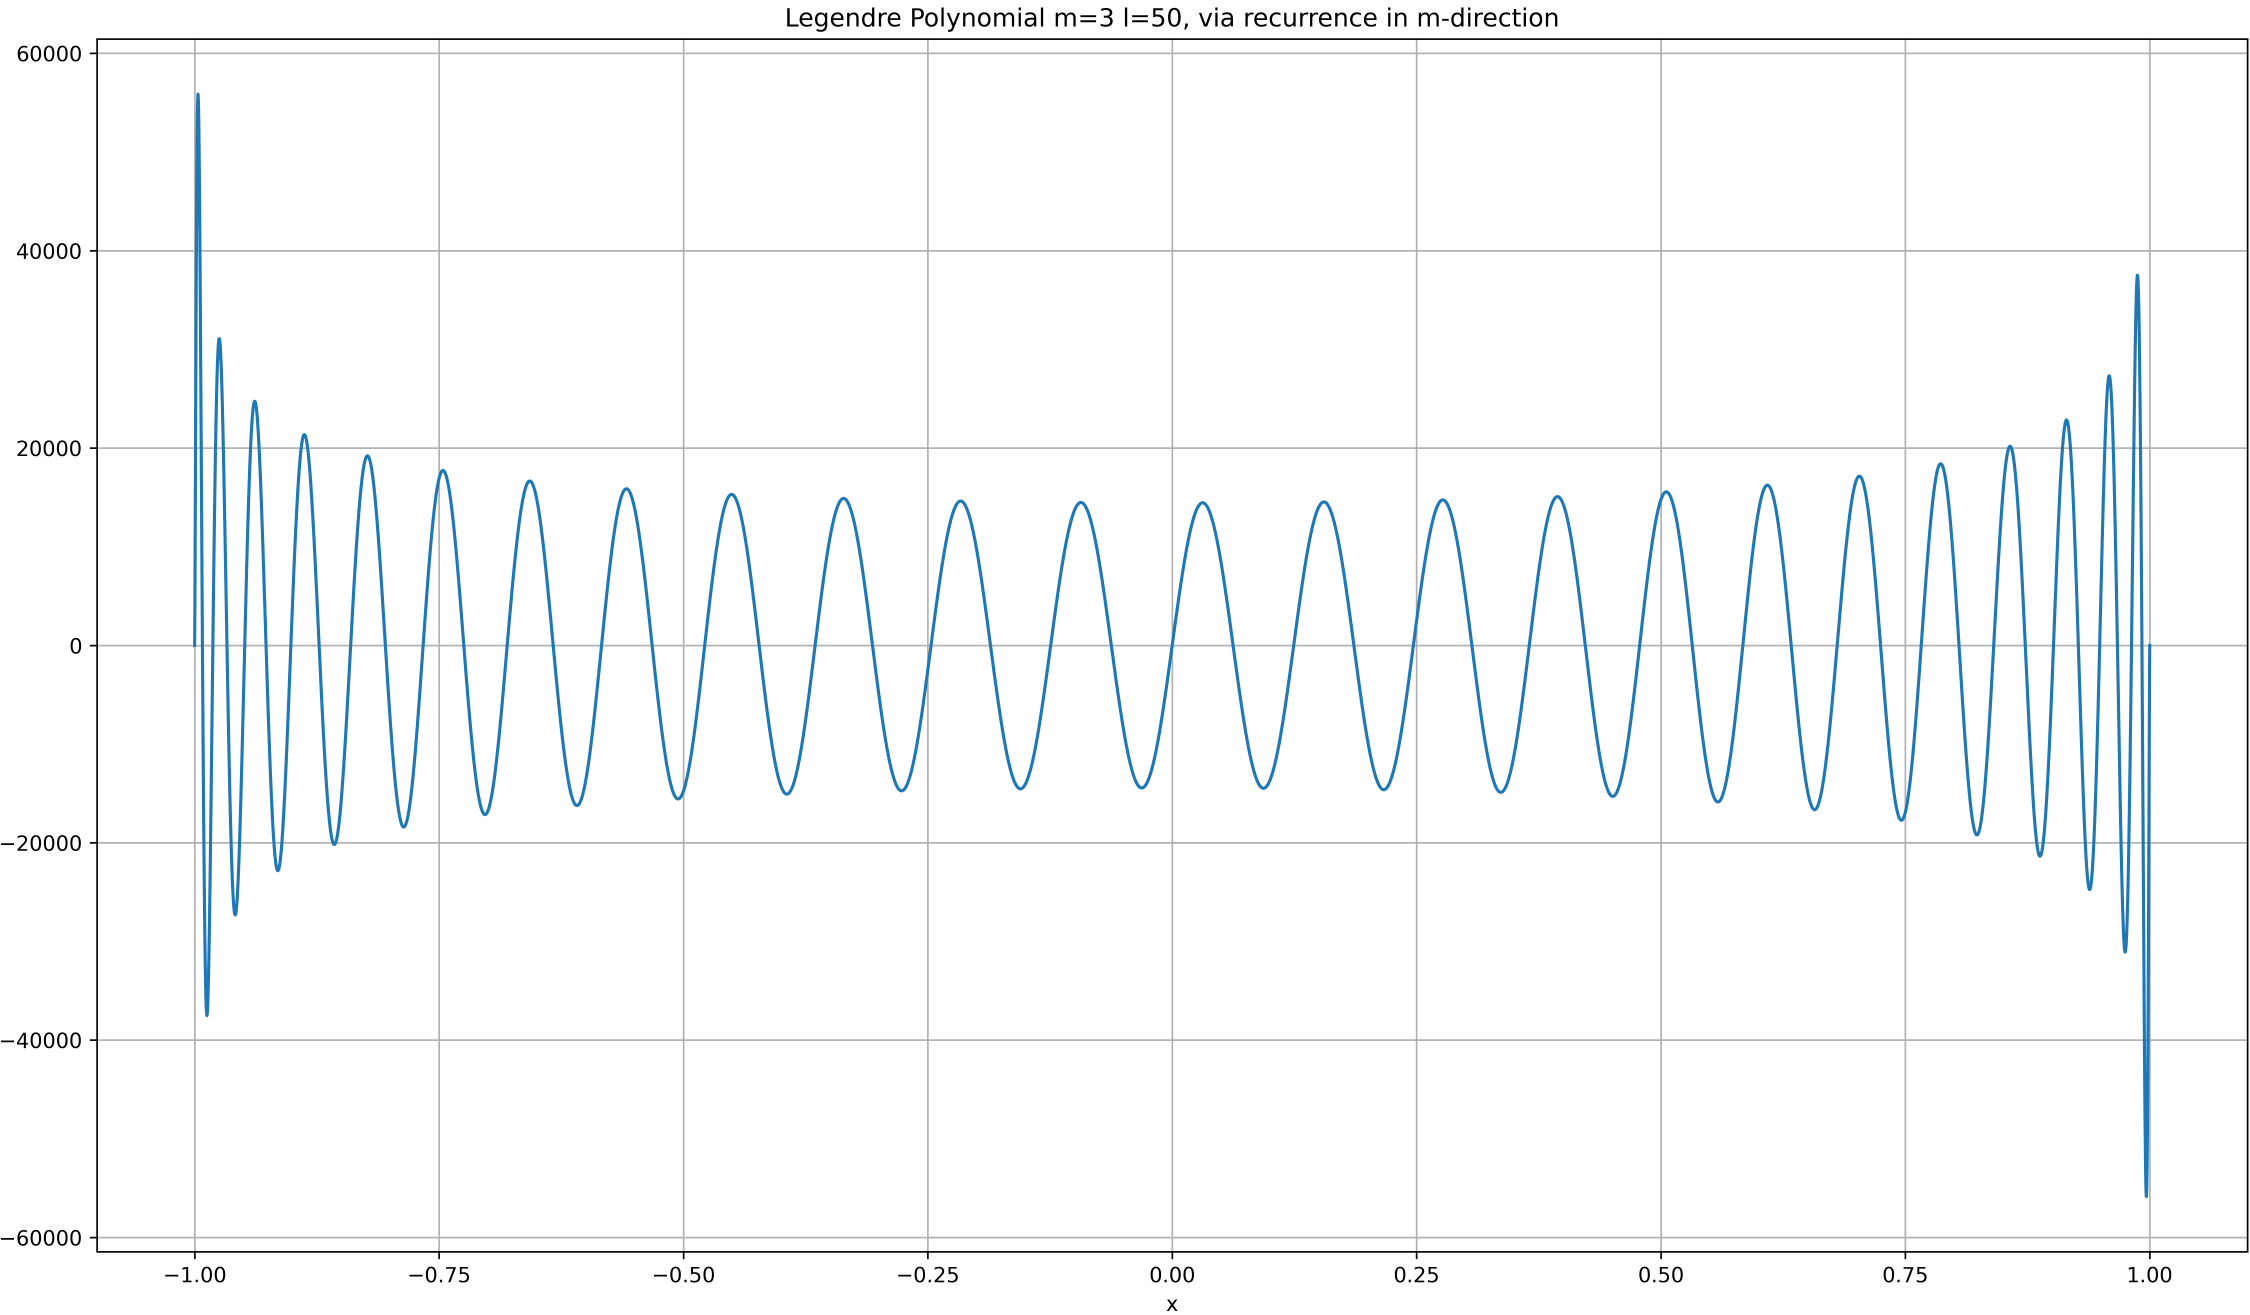
\includegraphics[width=1.0\linewidth]{papers/legendre/plots/plot_m_small.png}
\caption{Zugeordnetes Legendre-Polynom mit \texorpdfstring{$l=50$}{l=50} und \texorpdfstring{$m=3$}{m=3}, berechnet mit der Rekursionsformel in \texorpdfstring{$m$}{m}-Richtung.}
\label{legendre:fig:plot-m}
\end{figure}
Die beiden Graphen (Abbildungen \ref{legendre:fig:plot-l} und \ref{legendre:fig:plot-m}) zeigen, dass die Rekursionsformeln nicht die alleinige Ursache für die numerischen Instabilitäten des Legendre-Polynom-Graphen von Wolfram Alpha (Abbildung \ref{legendre:fig:wolframalpha}) sein können.
Trotzdem lohnt es sich die beiden Rekursionsformeln etwas genauer zu untersuchen.
Sie können nämlich mitverantwortlich sein für numerische Instabilitäten, indem sie numerische Fehler aus einer anderen Quelle begünstigen.
